\documentclass[a4paper,12pt]{article}
\usepackage[bahasa]{babel}
\usepackage{graphicx}
\usepackage{multirow}
\usepackage{enumitem}
\usepackage{listings}
\usepackage{adjustbox}
\graphicspath{ {./img/} }
\begin{document}
\title{Laporan Praktikum Statistika Pertemuan 11}
%\author{Aldzikri Dwijayanto Prathama \\ {\small 195410189}}
\author{Aldzikri Dwijayanto Prathama 
	\\195410189}
\makeatletter
\begin{titlepage}
	\begin{center}
		{\huge \bfseries \@title }\\[14ex]
		
\includegraphics[scale=.8]{logo}\\[4ex]
		{\large \@author}\\[20ex]
		{\large \bfseries {SEKOLAH TINGGI MANAJEMEN INFORMATIKA DAN KOMPUTER
				AKAKOM YOGYAKARTA}}
	\end{center}


%{\large \@date} 
\end{titlepage}
\makeatother
%\maketitle
\newpage
\tableofcontents
\newpage
\section{Pembahasan}
\begin{enumerate}[label=\textbf{\Alph*}.]
	\item \textbf{DISTRIBUSI BINOMIAL}\\
	Distribusi Binomial digunakan apabila sebuah proses sampling dilaksanakan
	sesusai dengan proses Bernoulli, yang memiliki ciri-ciri sebagai berikut:
	\begin{enumerate}
		\item Ada dua kejadian yang dapat terjadi dan saling asing pada setiap percobaan.\\ Untuk mudahnya, dua kejadian itu disebut sukses dan gagal.
		\item Urutan dari percobaan tersebut merupakan kejadian independen.
		\item Probabilitas sukses dinyatakan sebagai p, dimana nilai p ini tetap dari satu
		percobaan ke percobaan berikutnya atau dari satu kejadian ke kejadian
		lainnya.
	\end{enumerate}
	Pada distribusi Binomial, ada 3 nilai yang diperlukan yaitu : jumlah sukses (X),
	jumlah percobaan / observasi (n) dan probabilitas sukses dalam setiap percobaan (p).
	
	\item \textbf{DISTRIBUSI POISSON}\\
	Distribusi Poisson dapat digunakan untuk menentukan probabilitas dari sejumlah
	sukses yang ditentukan jika kejadian-kejadian berjalan dalam kurun waktu atau ruang
	kontinyu tertentu. Proses Poission hampir sama dengan proses Bernoulli hanya
	berbeda pada sifat kontinuitasnya. Pada distribusi Poisson hanya ada 1 nilai yang
	diperlukan, yaitu jumlah rata-rata sukses, dinyatakan sebagai x $\lambda$ . Distribusi Poisson
	efektif digunakan untuk jumlah pengamatan, n yang sangat besar, sementara
	probabilitas, p untuk satu kejadian sangat kecil (biasanya kurang dari 0,5).
\end{enumerate}

\newpage
\subsection{Praktik}
\begin{enumerate}[label=\textbf{\Alph*.}]
	
	\item \textbf{Menghitung probabilitas (p-value) data berdistribusi Poisson}
	\paragraph{Praktik 1\\}
	Pada distribusi Binomial dengan n = 5, p = 0.25, tentukan
	\begin{enumerate}[label=\alph*.]
		\item P(X = 0)\\
		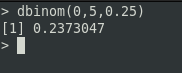
\includegraphics[scale=1]{praka1a}\\
		Pada praktik ini diketahui:\\
		X = 0\\
		n = 5\\
		p = 0.25\\
		maka pada praktik ini digunakan fungsi \texttt{dbinom}, karena pada praktik ini adalah mencari probabiliatas x dari n sampel dengan
		probabiltas sukses p atau mencari P(X = x), sehingga perintahnya:\\
		\texttt{dbinom(0,5,0.25)}\\
		dari output diatas diketahui P(x=0)=0.2373047
		
		\item P(X$\leq2$ )\\
		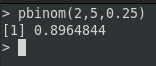
\includegraphics[scale=1]{praka1b}\\
		Pada praktik ini diketahui:\\
		X $\leq$2\\
		n = 5\\
		p = 0.25\\
		maka pada praktik ini digunakan fungsi \texttt{pbinom}, karena pada praktik ini adalah mencari probabiliatas kumulatif x dari n sampel
		dengan probabiltas sukses p atau mencari P(X < x), sehingga perintahnya:\\
		\texttt{pbinom(2,5,0.25)}\\
		dari output diatas diketahui P(x$\leq$2)=0.8964844	
	\end{enumerate}
\paragraph{Praktik 2\\}
Terdapat 10 mahasiswa dipilih secara acak dari populasi dimana 40\% adalah wanita.
\begin{enumerate}[label=\alph*.]
	\item Berapa probabilitas sebanyak satu dari mahasiswa tersebut yang dipilih adalah
	wanita?\\
	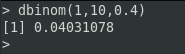
\includegraphics[scale=1]{praka2a}\\
	Diketahui:\\
	x = 1\\
	n = 10\\
	p = 0.4\\
	pada praktik ini digunakan fungsi \texttt{dbinom}, karena pada praktik ini adalah mencari probabiliatas x dari n sampel dengan
	probabiltas sukses p atau mencari P(X = x), sehingga perintahnya:\\
	\texttt{dbinom(1,10,0.4)}\\
	dari output diatas diketahui P(x=1)=0.04
	
	\item Berapa probabilitas paling banyak tiga orang dari mahasiswa tersebut yang dipilih
	adalah wanita?\\
	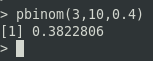
\includegraphics[scale=1]{praka2b}\\
	Pada praktik ini diketahui:\\
	X $\leq$ 3\\
	n = 10\\
	p = 0.4\\
	maka pada praktik ini digunakan fungsi \texttt{pbinom}, karena pada praktik ini adalah mencari probabiliatas kumulatif x dari n sampel
	dengan probabiltas sukses p atau mencari P(X < x), sehingga perintahnya:\\
	\texttt{pbinom(2,10,0.4)}\\
	dari output diatas diketahui P(x$\leq$3)=0.3822806
\end{enumerate}

\newpage
\item\textbf{Membangkitkan data berdistribusi Binomial\\}
Untuk membangkitkan sample sebanyak 10 dari distribusi Binomial dengan parameter n\\
= 5 dan p = 0,3\\
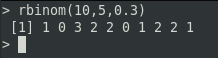
\includegraphics[scale=1]{prakb1}\\
Diketahui:\\
r =  10\\
n = 5\\
p = 0.3\\
Pada  praktik ini digunakan fungsi \texttt{rbinom}, karena praktik ini adalah membangkitkan r data berdistribusi binomial dari n sampel
dengan probabilitas sukses p. Maka perintahnya:\\
\texttt{rbinom(10,5,0.3)}\\
dari outputnya terdapat 1 0 3 2 2 0 1 2 2 1

\item \textbf{Mencari nilai x yang membatasi luas daerah(nilai peluang) distribusi Binomial\\}
Terdapat 10 mahasiswa dipilih secara acak dari populasi dimana 40\% adalah wanita.
Berapa banyak wanita yg terpilih dari mahasiswa tersebut, apabila diketahui peluang
terpilihnya 0,1 ?\\
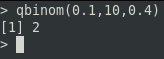
\includegraphics[scale=1]{prakc}\\
Diketahui:\\
P = 0.1\\
n = 10 \\
p = 40\%
Pada praktik ini digunakan perintah \texttt{qbinom} untuk mencari nilai x dari luasan (peluang) P berdistribusi binomial
dari n sampel dengan probabilitas sukses p. Maka perintahnya:\\
\texttt{qbinom(0.1,10,0.4)}\\
dari output diatas diketahui banyak wanita yg terpilih dari mahasiswa tersebut, apabila diketahui peluang
terpilihnya 0,1 adalah 2

\newpage
\item \textbf{Menghitung probabilitas (p-value) data berdistribusi Poisson}
\paragraph{Praktik 1\\}
Sebuah direktorat kemahasiswaan menyatakan bahwa mereka menerima keluhan
mahasiswa rata-rata 20 orang per hari. Tentukanlah
\begin{enumerate}[label=\alph*.]
	\item peluang bahwa pada suatu hari tidak ada mahasiswa yang datang\\
	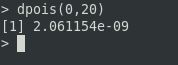
\includegraphics[scale=1]{prakd1a}\\
	Diketahui:\\
	n = 0 \\
	$\lambda$ = 20 \\
	Untuk mencari probabiliatas kumulatif x dengan rata-rata $\lambda$
	Atau P(X = x), digunakan perintah dpois, maka perintahnya:\\
	\texttt{dpois(0,20)}\\
	Sehingga diketahui probabiliatas kumulatif 0 dengan rata-rata 20 adalah 0,00000000206
	
	\item peluang mahasiswa yang datang paling banyak 14 orang.\\
	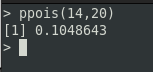
\includegraphics{prakd1b}\\
	Diketahui:\\
	x = 14\\
	$\lambda$ = 20\\
	Untuk mencari mencari probabiliatas kumulatif x dengan rata-rata $\lambda$
	Atau P(X $<$ x) gunakan fungsi \texttt{ppois}, sehingga perintahnya:\\
	\texttt{ppois(14,20)\\}
	jadi $P(X \leq 14) = 0,1048643$
\end{enumerate}

\newpage
\paragraph{Praktik 2\\}
Misalkan variabel random X berdistribusi Poisson dengan mean 3. Tentukan
\begin{enumerate}[label=\alph*.]
	\item probabilitas bahwa terdapat 5 partikel yang terdeteksi dalam suatu pengukuran\\
	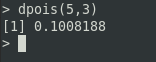
\includegraphics{prakd2a}\\
	Diketahui:\\
	n = 5 \\
	$\lambda$ = 3 \\
	Untuk mencari probabiliatas kumulatif x dengan rata-rata $\lambda$
	Atau P(X = x), digunakan perintah dpois, maka perintahnya:\\
	\texttt{dpois(5,3)}\\
	Sehingga diketahui probabiliatas kumulatif 5 dengan rata-rata 3 adalah 0,1008188
	
	\item probabilitas bahwa terdapat paling sedikit 2 partikel yang terdeteksi dalam suatu
	pengukuran\\
	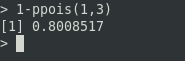
\includegraphics[]{prakd2b}\\
	Diketahui:\\
	X $\geq$ 2 = 1 - P(X $\leq$ 1)\\
	$\lambda$ = 3\\
	Untuk mencari mencari probabiliatas kumulatif x dengan rata-rata $\lambda$
	Atau P(X $<$ x) gunakan fungsi \texttt{ppois}, karena pada praktik ini yang dicari adalah X $\geq$ 2 maka perintahnya:\\
	\texttt{1 - ppois(1,3)\\}
	jadi $P(X \geq 2) = 1 - P(X \leq 1) = 0,8008517$
\end{enumerate}
\item \textbf{Membangkitkan data berdistribusi Poisson\\}
Untuk membangkitkan sample sebanyak 20 dari distribusi poisson dengan parameter
rata-rata $\lambda = 5$\\
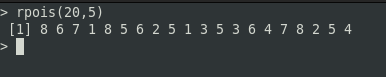
\includegraphics{prake}\\
Diketahui:\\
r = 20\\
$\lambda$ = 5\\
untuk membangkitkan r data berdidtribusi poisson dengan rata-
rata $\lambda$ gunakan perintah:\\
\texttt{rpois(20,5)}

\item \textbf{Mencari nilai x yang membatasi luas daerah(nilai peluang) distribusi Poisson}\\
Sebuah direktorat kemahasiswaan menyatakan bahwa mereka menerima keluhan
mahasiswa rata-rata 20 orang per hari. Tentukanlah banyaknya mahasiswa yg datang
mengeluh apabila diketahui probabilitas yg mengeluh 0,25
\end{enumerate}
\end{document}
